\chapter{Reele Zahlen, Euklidische Räume und Komplexe Zahlen}
\section{Elementare Zahlen}
\begin{tabular}{r l c c c}
Naturzahl & $\mathbb{N}$&$=$& $\{0,1,2,\dots\}$& addieren und multiplizieren\\
~& $\cap$ &~&~&~\\
LOOK TODO & $\mathbb{Z}$&$=$& $\{\dots ,-2,-1,0,1,2,\dots\}$& subtrairen\\
~& $\cap$ &~&~&~\\
Rationalzahlen & $\mathbb{Q}$&$=$& $\left\{ {\left. {\frac{p}{q}} \right|p,q \in \mathbb{Z},q\not  = 0} \right\}$& dividieren\\
\end{tabular}
\todo{Before set Z, can't read, page 22}\\
Viele gleichungen haben keine Lösung in $\mathbb{Q}$.
\subsubsection*{Satz 2.1}
Sei $p\in\mathbb{N}$ eine Primzahl. Dann hat $x^2=p$ keine Lösung in $\mathbb{Q}$
\subsubsection*{Beweis}
Zum Erinnerung zwei Natürlichen Zahlen $a$ und $b$ sind teilfrmd (oder relativ prim) wenn es keine Natürliche Zahl ausser der Eins gibt, die beiden Zahlen teilt. $$\left( (a,b)=1\right)\rightarrow\text{ grösste Gemeinsame Teiler}$$

\subsubsection*{Indirekter Beweis}
Wir nehmen an: es gibt $x=\frac{a}{b}\in \mathbb{Q}$ mit $x^2 =p$, wobei $a,b$ teilfremd und $\geq 1$ sind. Dann gilt $$a^2=pb^2$$ woraus folgt, dass $p$ $a$ teilt also ist $a=pk$, $k\in\mathbb{N}$ und somit $$a^2=p^2k^2=pb^2\Rightarrow pk^2=b^2$$ woraus folgt, dass $p$ $b$ teilt.

\section{Die Reelen Zahlen}
Wir werden jetzt das System von Axiomen beschreiben das die Menge der Reelen Zahlen ''eindeutig'' characterisiert. \\

Die Menge $\mathbb{R}$ der Reelen Zahlen ist mit zwei Verknüpfungen ''$+$'' (Addition) und ''$\cdot$'' (Multiplikation) versehen sowie mit einer Ordnungsrelation $\leq$. Die axiome werden wie folgt gruppiert:
\begin{enumerate}
\item \textbf{$\left( \mathbb{R},+,\cdot\right)$ ist ein Koerper}\\
Es gibt 2 Operationen (Zweistellige Verknüpfungen)
\begin{itemize}
\item $+:\mathbb{R}\times\mathbb{R}\rightarrow\mathbb{R}$\\
$(a,b)\rightarrow a+b$
\item $\times:\mathbb{R}\times\mathbb{R}\rightarrow\mathbb{R}$\\
$(a,b)\rightarrow a\cdot b$
\end{itemize}
und 2 ausgezeichnete Element 0 und 1 in $\mathbb{R}$ die folgenden Eigenschaften haben:\\
\begin{center}
\begin{tabular}{l r l r l}
Komutivität & A1) & $x+y=y+x$ & M1) & $x\cdot y=y\cdot x$ \\ 
Assoziativität & A2) & $(x+y)+z=x+(y+z)$ & M2) & $(xy)z=x(yz)$ \\
Neutrales Element & A3) & $x+0=x=0+x$ & M3) & $x\cdot 1=1\cdot x$\\
Inverse Element & A4) & $\forall x\in\mathbb{R}, \exists y\in\mathbb{R}$ & M4) & $\forall x\in\mathbb{R}, x\not =0$ \\
~&~& mit $x+y=0=y+x$ & ~& $ \exists y\in\mathbb{R}$ mit $xy=1=yx$
\end{tabular}
\end{center}
\todo{resize table}
und Die Multiplikation ist verträglich it der Addition im Sinne des Distributivitäts-Gesetz (D)$$\forall x,y,z\in\mathbb{R}:x(y+z)=xy+xz$$

\begin{itemize}
\item $( \mathbb{R},+)$ mit A1$\rightarrow$A4 ist eine Abelische Gruppe bezüglich der Addition
\item  $( \mathbb{R},+,\cdot)$ mit A1$\rightarrow$A4, M1$\rightarrow$M4 und D ist ein Zahlkörper. 
\end{itemize}

\subsubsection*{Bemerkung 2.2}
Eine Menge $G$ versetzen mit Verknüpfung $+$ und Neutrales Element $O$ die den obigen Eigenschaften A2$\rightarrow$A4 genügen heisst Gruppe.\\

Eine enge $K$ versetzen mit Verknüpfung $+,\cdot$ und Elementen $0\not =1$ die den obigen Eigenschaften 
A1$\rightarrow$A4, M1$\rightarrow$M4, D genügen heisst Körper. 

\subsubsection*{Folgerung 2.3}\todo{Add Big curly brackets to enum list, page 25}
Seien $a,b,c,d\in\mathbb{R}$ 
\begin{enumerate}[i)]
\item $a+b=a+c\Rightarrow b=c$ und $O$ is eindeutig, d.h. Falls $z\in\mathbb{R}$ der Eigenschaften $a+z=a$ $\forall a\in\mathbb{R}$ genügt, so folgt $z=0$
\item $\forall a,b\mathbb{R}$, $\exists !$ (eindeutig bestimmtes) $x\in\mathbb{R}:a+x=b$. Wir schreiben $x=b-a$ und $0-a=-a$ ist das additive Inverse zu $a$
\item $b-a=b+(-a)$
\item $-(-a)=a$
\item Falls $ab=ac$ und $a\not = 0\Rightarrow b=c$ und 1 ist eindeutig, d.h. falls $x\in\mathbb{R}$ der Eigenschaften $ax=a$ $\forall a\in\mathbb{R}$ genügt so folgt $x=1$
\item $\forall a,b\in\mathbb{R}$, $a\not =0$, $\exists !x\in\mathbb{R}:ax=b$. Wir schreiben $x=\frac{b}{a}$ und $\frac{1}/{a}=a^{-1}$ ist das Multiplikativ Inverse zu $a$.
\item Falls $a\not =0\Rightarrow {\left(a^{-1}\right)}^{-1}=a$ 
\item $\forall a\in\mathbb{R}$, $a\cdot 0=0$
\item Falls $ab=0$ dann folgt $a=0$ oder $b=0$
\end{enumerate}
\subsubsection*{Beweis 2.3}
\begin{enumerate}[i)]
\item Sei $a+b=a+c$\\ A4 $\Rightarrow\exists y\in\mathbb{R}:a+y=0$\\$a+b=a+c\Rightarrow y+(a+b)=y+(a+c)$\\$\Rightarrow (y+a)+b=(y+a)+c$\\$\Rightarrow 0+b=0+c \Rightarrow b=c$ \todo{add rules to top of arrows, page 26 top}\\
Nehmen wir an, dass es $0'\in\mathbb{R}$ gibt so dass $x+0'=x$, $\forall x\in\mathbb{R}$, d.h. es gibt eine zweite neutrale Element für $+$.\\

\noindent Dann $0+0'=0$ aber auch A3 $\Rightarrow 0+0=0\Rightarrow 0+0'=0+0\Rightarrow 0=0'$
\item Seien $a,b\in\mathbb{R}$, und sei $y\in\mathbb{R}$ mit $a+y=0$. Definieren wir $x:=y+b\Rightarrow a+x=a+(y+b)=(a+y)+b=0+b=b$\\
$\Rightarrow \exists$ mindestens eine Lösung der Gleichung $a+x=b$. Von i) folgt dass $x$ eindeutig bestimmt ist $a+x=b=a+x' \Rightarrow x=x'$
\item Seien $x=b-a$, $y=b+(-a)$. Wir Wollen beweisen dass $x=y$.\\

\noindent Aus i) wissen wir dass $b-a$ eine Lösung von $a+x=b$ $$y+a=\left( b+(-a)\right)+a=b+\left( (-a)+a\right)=b+0=0$$
$\Rightarrow y$ ist auch eine Lösung.\\
Weil die Lösung von $a+x=b$ ist eindeutig bestimmt, ist $y=x$
\item
\item
\item
\item
\todo{ASK FOR BEWEISE; PAGE 27 TOP}
\item $\forall a\in\mathbb{R}$, $a\cdot 0=0$\\
$a\cdot 0=a(0+0)=a\cdot 0+a\cdot 0\Rightarrow a\cdot 0=0$
\item $ab=0\Rightarrow a=0$ oder $b=0$\\
Wir nehmen an: $a\not=0$ mit \todo{?multipli? page 27 middle to top} Inversen $a^{-1}$, ( $a^{-1}$ existiert mittels M4). So folgt $b=1\cdot b=\left( a^{-1}\cdot a\right)b=a^{-1}(a\cdot b)=a^{-1}\cdot 0=0$
\end{enumerate}
\item Ordnungsaxiome $\leq$\\
Auf $\mathbb{R}$ gibt es eine Relation, $\leq$, genanten Ordnung, die folgenden Eigenschaften genügt
\begin{enumerate}
\item Reflexität: $\forall x\in\mathbb{R}$, $x\leq x$
\item Transitivität: $\forall x,y,z\in\mathbb{R}$: $x\leq y\land y\leq z\Rightarrow x\leq z$
\item Identivität: $\forall x,y\in\mathbb{R}$, $(x\leq y)$ und $(y\leq x)\Rightarrow x=y$
\item Die Ordnung ist total: $\forall x,y\in\mathbb{R}$ gilt entweder $x\leq y$ oder $y\leq x$ 
\end{enumerate}
Die Ordnung ist konsistent mit $+$, und $\cdot$
\begin{enumerate}
\item $x\leq y\Rightarrow x+z\leq y+z$\hspace{10mm}$\forall x,y,z\in\mathbb{R}$
\item $x,y\geq 0\Rightarrow xy\geq 0$
\end{enumerate}
Mit $\leq$ hat man auch$\geq,<,>$. Wir Verzichten auf eine Auflistung aller Folgerungen und beschränken uns auf einzige wichtige Folgerungen.
\subsubsection*{Folgerungen 2.4}
\begin{enumerate}[i)]
\item $x\leq 0$ und $y\leq 0 \Rightarrow xy\geq 0$
\item $x\leq 0$ und $y\geq 0\Rightarrow xy\leq 0$
\item $x\leq y$ und $z\geq 0\Rightarrow xz\leq yz$
\item $1>0$
\item $\forall x\in\mathbb{R}$\hspace{10mm}$x^2\geq 0$
\item $0<1<2<3<\dots$
\item $\forall x>0: x^{-1}>0$
\end{enumerate}
\{Annahme: $x^{-1}\leq 0$. Nach Multiplikation mit $x>0$ folgt (mittels ii) $1=x^{-1}\cdot x\leq 0\cdot x=0$\}
\subsubsection*{Bemerkung 2.5}
$\leq$ auf \todo{What? page 28 bottom} genügt den obigen Eigenschaften. Die entscheidende weitere Eigenschaft von $\mathbb{R}$ ist das.
\item Ordnungsvollständigkeit\\
Vollständigskeitaxiom:\todo{Check for layout issues with title}\\
Seien $A,B\subset\mathbb{R}$ nicht leere Teilmenge von $\mathbb{R}$, so dass $a\leq b$ für alle $a\in A,b\in B$. Dann gibt es $c\in\mathbb{R}$ mit $a\leq c\leq b$\hspace{5mm} $\forall a\in A,b\in B$
\subsubsection*{Bemerkung 2.6}
\todo{What? page 29 bottom} erfüllt dieses Eigenschaft nicht!\\


Seien $$A=\{x\in\mathbb{Q}\mid x\geq 0, x^2\leq 2\}$$ $$B=\{y\in Q\mid y\geq 0, y^2 \geq 2\}$$ 

Dann gilt $a\leq b$ $\forall a\in A$ $b\in B$. ABer ein $c\in\mathbb{Q}$, mit $a\leq c\leq b$ würde dann $c^2=2$ erfüllen! In Satz 2.1 haben wir gesehen dass $x^2=p$ keine Lösung in $\mathbb{Q}$ hat. \\

Wir definieren jetzt für $x,y\in\mathbb{R}$ \[\max \{ x,y\}  = \left\{ {\begin{array}{*{20}{c}}
{x\text{ falls }y \le x}\\
{y\text{ falls }x \le y}
\end{array}} \right.\] Insbesondere ist der Absolutbetrag einer zahl $x\in\mathbb{R}, \left| x \right|$ $$\left| x \right|:\max \{x,-x\}$$ Für diesen gilt folgender Wichtiger Satz
\subsubsection*{Satz 2.7}
\begin{enumerate}[i)]
\item $\left| {x + y} \right| \le \left| x \right| + \left| y \right|$ (Dreiecks Ungleichung)
\item $\left| {xy} \right| = \left| x \right|\left| y \right|$
\end{enumerate}
\subsubsection*{Beweis 2.7}
\begin{enumerate}[i)]
\item $x \le \left| x \right|, - x \le \left| x \right|$\\$y \le \left| y \right|, - y \le \left| y \right|$\\und $x+y\leq  \left| x \right| +  \left| y \right|, - (x + y) \le \left| x \right| + \left| y \right|$ \\ woraus $\left| {x + y} \right| \le \left| x \right| + \left| y \right|$ folgt
\item ASK FOR BEWEIS\todo{ASK FOR BEWEIS}
\end{enumerate}

\subsubsection*{Satz (Young)}
Für alle $a,b\in\mathbb{R}$. $\delta >0$ gilt $2\left| {ab} \right| \le \delta {a^2} + \frac{{{b^2}}}{\delta }$
\end{enumerate}

\section{Infimum und Supremum}
In Zusammenhang mit der Ordnung führen wir einige Wichtige Definitionen ein:

\begin{framed}
\centerline{\textbf{\textbf{Definition 2.8}}}
\noindent Sei $\Romanbar{X}\subset\mathbb{R}$ eine Teilmenge 
\begin{enumerate}[\indent a)]
\item $\Romanbar{X}$ ist nach oben beschränkt falls es $c\in\mathbb{R}$ gibt $x\leq c, \forall x\in X$. Jeder derartige $c$ heisst eine Obere Schranke für $\Romanbar{X}$.
\item $\Romanbar{X}$ ist nach unten beschränkt, falls es $c\in\mathbb{R}$ gibt, mit $x\geq c$, $\forall x\in X$. Jeder derartige $c$ heisst untere Schranke für $\Romanbar{X}$.
\item $X$ ist beschränkt falls es nach oben und unten beschränkt ist.
\item Ein element $a\in\Romanbar{X}$ ist ein maximales Element (oder Maximum) von $\Romanbar{X}$ falls $x\leq a$, $\forall x\in\Romanbar{X}$. Falls ein Maximum (resp. minimum) existiert, wird es mit $\max\Romanbar{X}$ ($\min\Romanbar{X}$) bezeichnet. Falls $\Romanbar{X}$ keine obere schränke hat, ist $\Romanbar{X}$ nach oben unbeschränkt (analog für obere sch.).
\end{enumerate}
\end{framed}
\subsubsection*{Beispiel 2.9}
\begin{enumerate}
\item $A=\{x\in\mathbb{R}\mid x>0\}$ ist nach oben unbeschränkt. $A$ ist nach unten beschränkt. Jedes \todo{WHAT? Page 32 top}$\leq 0$ ist eine untere Schranke. 
\item $B=\lbrack 0,1\rbrack$ ist nach oben und nach unten beschränkt. \begin{itemize}
\item 0 ist ein minimum von $B$
\item 1 ist ein maximum von $B$ 
\end{itemize}
\item $C=\lbrack 0,1)$ ist nach oben und nach unten beschränkt, $0=\min(A)$. $C$ hat kein Maximum. 
\end{enumerate}
Folgender Satz ist von Zentraler Bedeutung und eine Folgerung der Ordnungsvollständigkeitaxiom.

\subsubsection*{Satz 2.10}
\begin{enumerate}[i)]
\item Jede nicht leere nach oben beschränkte Teilmenge $A\subset B$ besitzt eine kleinste obere Schranke $c$. Die Kleinste obere schranke $c$ ist eindeutig bestimmt und heisst Supremum von $A$, mit $\sup A$ bezeichnet. 
\item Jede nicht leere nach unten beschränkt Teilmenge $A\subset\mathbb{R}$ besitzt eine grösste untere Schranke $d$ und heisst Infimum von $A$, mit $\inf A$ bezeichnet.
\end{enumerate}
\subsubsection*{Beweis}
\begin{enumerate}[i)]
\item Sei $\emptyset\not=A\subset B$ nach oben beschränkt. Sei $B:=\{b\in\mathbb{R}\mid b$ ist obere Schranke für $A\}$. Dann $B\not=\emptyset$ und $a\leq b$, $\forall a\in A$ $b\in B$\\

Mit Ordnungsvollständigkeit Axiom folgt die Existens eine Zahl $c\in\mathbb{R}$ mit $a\leq c\leq b$ $\forall a\in A$, $b\in B$.\\

Es ist klar dass $c$ ist eine obere Schranke für $A$. Also $c\in B$. Da $c\leq b$ $\forall b\in B$, ist $c$ die kleinste obere Schranke für $A$. Hierdurch $c$ ist eindeutig bestimmt.\\

(Seien $c$ und $c'$ zwei Supremum von $A$, $c$ ist die kleinste obere Schranke und $c'$ ist eine obere Schranke $\Rightarrow c\leq c'$. Das gleiche Argument mit $c$,$c'$ ausgetauscht liefert $c'\leq c$)
\item Sei $A$ nach unten beschränkte, nicht leere Menge. Sei $-A:=\{ -x\mid x\in A\}$ die Menge der additive Inversen von $A$. Dann $-A\not=\emptyset$ und nach oben beschränkt. i) $\Rightarrow \exists s=\sup (-A)\Rightarrow -s$ ist das Infimum von $A$ 
\end{enumerate}

\subsubsection*{Korollar 2.11}
\begin{enumerate}
\item Falls $E\subset F$ und $F$ nach oben beschränkt ist, gilt $\sup E\leq \sup F$ 
\item Falls $E\subset F$ und $F$ nach unten beschränkt ist, gilt $\inf F\leq \inf E$ 
\item Falls $\forall x\in E$, $\forall y\in F$ gilt $x\leq y$ dann folgt $\sup E\leq\inf F$ 
\item Seien $E,F\not=\emptyset$, $E,F,\subset\mathbb{R}$, $h\in\mathbb{R}$, $h>0$ \todo{page is clipped, page 34 bottom}
\begin{enumerate}[(i)]
\item Falls $E$ ein sup. besitzt $\Rightarrow \exists x\in E$ mit $x>\sup E$\todo{can't read, is it E-h? page 34 bottom}
\item Falls $E$ ein Inf besitzt $\Rightarrow \exists y\in : y<\inf E+h$. Das Supremum, $\sup\Romanbar{X}=\sigma$ der Menge $\Romanbar{X}$ ist folgendermassen charakterisiert: Es gibt in $\Romanbar{X}$ keine Zahlen $>\sigma$; aber für jede Toleranz $h>0$ gibt es in $\Romanbar{X}$ Zahlen $>\sigma -h$ 


\begin{center}
\begin{tikzpicture}

\draw [black] (0.5,-0.1) rectangle (2,0.1); 
\draw [black] (2.5,-0.1) rectangle (2.8,0.1); 
\draw [black] (3.5,-0.1) rectangle (3.8,0.1); 
\draw [black] (3.9,-0.1) rectangle (4.2,0.1); 
\draw [black] (4.5,-0.1) rectangle (4.9,0.1); 
\draw [black] (4.95,-0.1) rectangle (5.35,0.1); 
\draw(5.35,0.5)--(5.35,-0.5);
\draw(5.7,0.5)--(5.7,-0.5);
\draw [black] (5.35,-0.1) rectangle (5.55,0.1); 
\draw [black] (5.58,-0.1) rectangle (5.68,0.1); 
\node[anchor=west,scale=0.7] at (5.8,-0.3){$\sigma =\sup M$};

\draw [black,decorate,decoration={brace,amplitude=2pt,mirror},xshift=0.4pt,yshift=-0.4pt](5.35,-0.5) -- (5.7,-0.5) node[black,midway,yshift=-8] {\footnotesize $h$};
\draw[](0,0)--(6,0);

\draw[](0,-2)--(6,-2);

\begin{scope}[yscale=1,xscale=-1,xshift=-170]
\draw [black] (0.5,-2.1) rectangle (2,-1.9); 
\draw [black] (2.5,-2.1) rectangle (2.8,-1.9); 
\draw [black] (3.5,-2.1) rectangle (3.8,-1.9); 
\draw [black] (3.9,-2.1) rectangle (4.2,-1.9); 
\draw [black] (4.5,-2.1) rectangle (4.9,-1.9); 
\draw [black] (4.95,-2.1) rectangle (5.35,-1.9); 
\draw [black] (5.35,-2.1) rectangle (5.55,-1.9); 
\draw [black] (5.58,-2.1) rectangle (5.68,-1.9); 
\end{scope}
\draw(0.625,-1.5)--(0.625,-2.5);
\draw(0.295,-1.5)--(0.295,-2.5);
\draw(5.7,0.5)--(5.7,-0.5);

\draw [black,decorate,decoration={brace,amplitude=2pt,mirror},xshift=0.4pt,yshift=-0.4pt](0.295,-2.5) -- (0.625,-2.5) node[black,midway,yshift=-8] {\footnotesize Inf F};
\end{tikzpicture}
\end{center}



Es gibt in $\Romanbar{X}$ keine Zahlen $<\inf\Romanbar{X}=$\todo{faded color, can't read, page 34.1 middle to bottom} aber für jede Toleranz $h>0$ gibt es in $\Romanbar{X}$ Zahlen $<\inf \Romanbar{X}+h$
\item Sei $E+F=\{ e+f:e\in E,f\in F\}$. Falls $E$ und $F$ ein Sup. besitzen $\Rightarrow E+F$ besitzt ein Sup und $\sup (E+F)=\sup(E)+\sup(F)$. (Analog mit Inf.) 
\end{enumerate}
\end{enumerate}
\subsubsection*{Beweis}
\todo{Ask for full Beweis!!}
\subsubsection*{Beispiel}
\begin{enumerate}
\item $E=(+\infty,2)\subset F(-\infty,4\rbrack$\\
$\sup E=2, \sup F=4=\max F$\\
$E$ hat kein Max: $\sup E\leq \sup F$
\item $G:\lbrack 4,5)\subset H=(3,6)$\\
$\min E=\inf G=4\geq \inf H=3$
\item $K=(3,\infty)$, $E=(-\infty,2)$\\
$\forall x\in E$, $y\in K$ gilt $x\leq y$\\
$2=\sup E\leq 3=\inf K$
\item $A\{\sin x\mid x\in\mathbb{R}\}$\\
$\inf S=-1=\min A$\\
$\sup A=1=\max A$
\item $A=\{\left( 1+\frac{1}{n}\right)^n\mid n\in\mathbb{N} \}$. Wir werden sehen dass $A$ ist nach unten und nach unten beschränkt. \\
$\inf A=\min A=2$, $\sup A=e=2.718\dots$
\underline{Vereinbarung}\todo{Check for better layout}\\
Für nach oben unbeschränkte Mengen $A\not=\emptyset$ setzen wir $\sup A=\infty$ unendlich. Analog fèr nach unten unbeschränkte Menge $\emptyset\not= A$ setzen wir $\inf A=-\infty$ 
\end{enumerate}
Die Folgende Satz zeigt wie die Ordnungsvollständigkeit von $\mathbb{R}$ die Lösbarkeit gewisser Gleichungen in $\mathbb{R}$ garantiert.

\subsubsection*{Satz 2.12}
Für jedes $x>0$ gibt es genau ein $y>0$ mit $y^2=x$. Diese Lösung wird mit $\sqrt{x}$ bezeichnet.\\

(Im Allgemein: Für jedes $x>0$ und $n\geq 1$, $n\in\mathbb{R}$ gibt es genau ein $y>0$ mit $y^2=0$. Diese Lösung wird mit $\sqrt[n]{x}$ bezeichnet)
\subsubsection*{Beweis}
Sei $x>1$, und $A:=\{ z\in\mathbb{R}\mid z>0$ mit $z^2\leq x\}$. Dann ist $A$ nach oben beschränkt und $A\not=\emptyset (1\in A)$. \todo{Not sure, page 35 bottom}$\Rightarrow A$ besitzt ein Supremum. \\
Sei $y:=\sup A$. Wir zeigen dass $y^2=x$
\begin{itemize}
    \item Schnitt 1: Annahme $y^2<x$. \\ 
    Sei $0\leq h\leq 1$.  Wir nehmen $$\left( y+h\right)^2=y^2+2hy+h^2$$
    $$=y^2+h(2y+h)$$
    $$\leq y^2+h(2y+1)$$
    $$=y^2 +h\left( (y+1)^2 -y^2\right)$$
    Weil $y^2<x$ ist, $\frac{x-y^2}{(y+1)^2-y^2}>0$ und daher gibt es $h\in\mathbb{R}$, $h>0$, $h\leq\frac{x-y^2}{(y+1)^2-y^2}$ (sei $h=\min \{1,\frac{x-y^2}{2x+1}\}$)\\
    
    Für solche $h$ gilt $$(y+h)^2\leq y^2 + \left( \frac{x-y^2}{(y+1)^2-y^2}\right)\left( (y+1)^2 -y^2\right)=$$\todo{chopped result, page 35.1} Also $y+h\in A$ und $y+h>y$. Ein widerspruch: $y$ ist eine obere schranke für $A$, d.h., $z<y$\\$\Rightarrow y^2\geq x$ Analog beweist man $y^2\leq x$
    \item Schnitt 2: Annahme $y^2>x$\\
    Sei $h=\frac{y^2-x}{2y}\not=0$ 
    $$(y-h)^2=y^2-2hy+h^2>y^2-2hy=y^2 -(y^2-=x$$\todo{Chopped, page 35.2 top}
    $\Rightarrow y-h$ ist eine Obere Schranke für $A$
    $$\left( \forall z \in A, z^2\leq x\text{\newline Da }(y-h)^2>x \text{ ist, } (y-h)^2>x\geq z^2\text{\newline Damit } y-h>z, \forall z \in A\right)$$\todo{break into three lines, page 35.2}
    Aber $y-h<y$, wiederspruch zur Minimalität von y.
\end{itemize}
Falls $0<x<1$, dann $\frac{1}{x}>1$\\
$\Rightarrow \exists u\in\mathbb{R}$, mit $u^2=\frac{1}{x}$\\
Somit $\left( \frac{1}{u}\right)^2=x$ und $y=\frac{1}{u}$ ist eine Lösung von $y^2=x$.\\

Zum Abschluss dieses Themas erwähren wir noch eine Wichtige Eigenschaft der Reelen Zahlen

\subsubsection*{Satz 2.13 (Archimedische Eigenschaft)}
Zu jeder Zahl $0<b\in\mathbb{R}$ gibt es ein $n\in\mathbb{N}$ mit $b<n$.
\subsubsection*{Beweis (Indirekt)}
Andernfalls gibt es $b\in\mathbb{R}$ mit $n\leq b$, $\forall n\in\mathbb{N}$ $$\left( \lnot\left(\exists n\in\mathbb{N}:b<n\right)=\left(\forall n\in\mathbb{N}:b\geq n\right)\right)$$
Dann ist $b$ eine obere Schranke für $\mathbb{N}$ und es existiert $c=\sup\mathbb{N}\in\mathbb{R}$. Mit $n\in\mathbb{R}$ ist jedoch auch $n+1\in\mathbb{N}$.\\
Also: $n+1\leq c$, $\forall n\in\mathbb{N}$. Somit folgt $n\leq c-1$, $\forall n\in\mathbb{N}$ ein widerspruch zur minimalität von \todo{Chopped content, page 36 bottom}.

\subsubsection*{Korollar 2.14}
\begin{enumerate}
    \item Seien $x>0$ und $y\in\mathbb{R}$ gegeben. Dann gibt es $n\in\mathbb{Z}$ mit $y<nx$
    \item Falls $x,y,a\in\mathbb{R}$ die ungleichkeiten $a\leq x\leq a+\frac{y}{n}$, $\forall n\in\mathbb{N}$ erfüllen, ist $x=a$.
\end{enumerate}
\subsubsection*{Beweis}

\begin{enumerate}
    \item ASK FOR BEWEIS\todo{Ask for beweis}
    \item $a<x\Rightarrow x-a>0\Rightarrow \exists n\in\mathbb{N}$\\
$\Rightarrow x>a+\frac{y}{n}$ Widerspruch
\end{enumerate}
Wir wissen dass gewisse Gleichungen in $\mathbb{R}$ Lösbar ist: z.B. $y^2=a$, $\forall a>0$. Aber man kann nicht alle GLeichugen in $\mathbb{R}$ lösen, z.B. $x^2+1=0$. Da für alle $x\in\mathbb{R}$, $x^2>0$, ist $x^2=-1$ nicht lösbar. Um eine Lösung für diese Gleichung zu finden, müssen wir die komplexen Zahlen betrachten.\\

\noindent Zuerst, werden wir die Euklidischen Räume $\mathbb{R}^n$ einführen
\section{Euklidische Räume}
Von der Mengentheorie können wir die Kartesische Produkt zweier Mengen; es Lässt sich ohne schwierigkeiten zu endlichen Familien $A_1,\dots ,A_n$ verallgemeinen; nähmlich $$A_1\times\dots\times A_n:=\{\left(x_1,\dots ,x_n\right):x_i\in A_i \}$$ ist die Menge der geordneten $n-$tuple von Elementen aus $A_1,\dots ,A_n$.\\

Für beliebige $n\geq 1$ betrachten wir $\mathbb{R}^n:=\underbrace{\mathbb{R}\times\dots\times\mathbb{R}}$\todo{Add n-mal to underbrace}  und untersuchen Seine Struktur. Auf $\mathbb{R}^n$ haben wir zwei Verknüpfungen
\begin{enumerate}
    \item $+:\mathbb{R}^n\times\mathbb{R}^n\rightarrow\mathbb{R}^n$ Addition.\\
$\left( {\underbrace {\left( {{x_1}, \ldots ,{x_n}} \right)}_x,\underbrace {\left( {{y_1}, \ldots ,{y_n}} \right)}_y} \right) \to \underbrace {\left( {{x_1} + {y_1}, \ldots ,{x_n} + {y_n}} \right)}_{{\text{Komponentenweise Addition}}}$. Dann ist $\left( \mathbb{R}^n,+\right)$ eine Abelische Gruppe, mit $0:=(0,\dots,0)$ aln neutrales Element
\item $\cdot:\mathbb{R}\times\mathbb{R}^n\rightarrow\mathbb{R}^n$ Skalarmultiplikation.\\
$(\lambda,x)\rightarrow\lambda\cdot x:=(\lambda x_1,\dots,\lambda x_n)$. Dann gelten die folgende Eigenschaften: $\forall x,y\in\mathbb{R}^n,\forall \alpha,\beta\in\mathbb{R}$ 
\begin{enumerate}
\item Distributivität: $\left( \alpha+\beta\right) x=\alpha x+\beta x$
\item Distributivität: $\alpha\left(x+y\right) = \alpha x+\alpha y$
\item Assoziativität: $\left( \alpha\beta\right) x=\alpha\left( \beta\right) x$
\item Einzelelement: $1\cdot x=x$
\end{enumerate}
\end{enumerate}

\begin{framed}
\centerline{\textbf{Definition 2.15}}
\noindent Eine Menge $\mathbb{V}$ ,it $+,\cdot$ und $0\in\mathbb{V}$ so dass $\left(\mathbb{V},+\right)$ eine Abelische Gruppe mit Neutralen Element 0 ist und zudem (a)-(d) gelten nennt sich ein Vektorraum über den Körper $\mathbb{R}$ und seine Elemente heissen Vektoren
\end{framed}
Also ist $\mathbb{R}^n$ ein Vektorraum. In der Linearen Algebra führt man dann Begriffe wie Basis usw. ein. Die Standard basis von $\mathbb{R}^n$ ist die Menge $\{e_1,e_2,\dots,e_n \}$ wobei $e_i:=\{0,\dots,0,1,\dots,0\}$ \\

Jeder Vektor $x=\left(x_1,\dots,x_n \right)\in\mathbb{R}$ besitzt eine eindeutige Darstellung $x=\sum x_ie_i$ bezüglich der Standardbasis.

\begin{framed}
\centerline{\textbf{Definition 2.16}}
\begin{enumerate}
\item Das Skalarprodukt zweier Vektoren $x=\left(x_1,\dots,x_n \right),y=\left(y_1,\dots,y_n \right)$ ist die durch \[ < x,y > : = \sum\limits_{i = 1}^n {{x_i}{y_i}} \] definierte reele Zahl\\ $<\cdot,\cdot>=\mathbb{R}^n\times\mathbb{R}^n\rightarrow\mathbb{R}$ (orthogonal)
\item Falls $<x,y>=0$ heissen $x$ und $y$ senkrecht aufeinander. $<\cdot,\cdot>$ besitzt folgende Eigenschaften
\begin{enumerate}
\item Symmetrie: $<x,y>=<y,x>$
\item Linearität: $<x,\alpha y+\beta z>=\alpha <x,y>+\beta <x,z>$
\item Positivität: $<x,x>\geq 0$ mit Gleicheit genau dann wenn $x=0$
\end{enumerate}
\end{enumerate}
\end{framed}

\begin{framed}
\centerline{\textbf{Definition 2.17}}
\noindent Die Norm $\left|\left| x\right|\right|$ eines Vektors ist: $$\left|\left|x\right|\right| := \sqrt{<x,x>}=\sqrt{\sum\limits_{i = 1}^n {{x_i}}}$$ wird oft als Länge interpretiert.
\subsubsection*{Beispiel 2.18}
\begin{itemize}
    \item

$\left|\left|(1,2)\right|\right|=\sqrt{1+4}$ 


\begin{center}
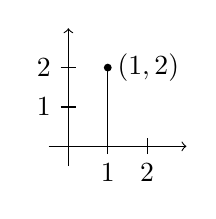
\begin{tikzpicture}[scale=0.5]
\draw[->](-0.5,0)--(3,0);
\draw[->](0,-0.5)--(0,3);
\draw(1,0)--(1,2);
\draw(-0.2,1)--(0.2,1);
\draw(-0.2,2)--(0.2,2);
\draw(1,-0.2)--(1,0.22);
\draw(2,-0.2)--(2,0.2);
\node[anchor=west] at (1,2){$(1,2)$};
\node[anchor=east] at (-0.2,2){$2$};
\node[anchor=east] at (-0.2,1){$1$};
\node[anchor=north] at (1,-0.2){$1$};
\node[anchor=north] at (2,-0.2){$2$};

\node[circle,fill=black,inner sep=1] (a) at (1,2) {};
\end{tikzpicture}
\end{center}










    \item $\left|\left|(1,1,1)\right|\right|=\sqrt{3}$
\begin{center}
\begin{tikzpicture}[scale=1,smooth,
                        line cap=round,line join=round]
    %% Define coordinate labels.
    % t(op) and b(ottom) layers
    \path \foreach \layer/\direction in {b/{0,0,0},t/{0,1,0}} {
        (\direction)
        \foreach \point/\label in {{0,0,0}/ll,{1,0,0}/lr,{1,0,-1}/ur,{0,0,-1}/ul} {
            +(\point) coordinate (\layer\label)
        }
        ($(\layer ll)!0.5!(\layer ur)$) coordinate (\layer md)
    };

    % Put text next to the labels as requested.
    % Funilly enough we need to set fill opacity to 1.


    % Draw left cube.
    \fill (0,0,-1) circle (1pt);
    \foreach \direction in {(0,0,1),(0,1,0),(1,0,0)} {
        %\draw[dashed,black] (bul) -- + \direction;
    }
    \draw (bll) -- (blr) -- (tlr) -- (tll) -- cycle;
    \draw (blr) -- (bur) -- (tur) -- (tlr) -- cycle;
    \draw (tll) -- (tlr) -- (tur) -- (tul) -- cycle;
    \foreach \point in {bll,blr,bur,tll,tlr,tul,tur} {
        \fill[fill opacity=1] (\point) circle (1pt);
    }
\draw[->](0,0,-1)--(0,0,1);
\draw[->](0,0,-1)--(0,2,-1);
\draw[->](0,0,-1)--(2,0,-1);
\draw[->,thick](2.2,1.5,1)--(1.1,1,0);
\node[anchor=west,scale=0.8] at (2.2,1.5,1){$(1,1,1)$};

    \end{tikzpicture}
\end{center}

    \item $\left|\left|e_i\right|\right|=1$, $<e_i,e_j>=0$. $e_i \perp e_j$\\
$\{e_1,e_2,\dots,e_n\}$ ist eine orthonormale Basis. Sie sind orthogonal und auf Länge 1 normiert.
\end{itemize}
\end{framed}
Die erste wichtige Eigenschaft eines Skalaprodukts ist
\subsubsection*{Satz 2.19 (Cauchy-Schwarz)}
$\forall x,y\in\mathbb{R}^n$ gilt $\left| <x,y>\right| \leq \left|\left| x\right|\right| \left|\left| y\right|\right|$ und $$\left| <x,y>\right|=\left|\left| x\right|\right| \left|\left| y\right|\right|\Leftrightarrow \exists\lambda\in\mathbb{R}: x=\lambda y$$

Die Euklidische Norm hat die Eigenschaften
\subsubsection*{Satz 2.20}
\begin{itemize}
    \item $\left|\left| \alpha x\right|\right|=\left|\alpha\right|\left|\left| x\right|\right|$ (Homogenität)
    \item $\left|\left| x+y\right|\right| \leq \left|\left| x\right|\right| + \left|\left| y\right|\right|$ (Dreiecks Ungleichung)
\end{itemize}

\subsubsection*{Beweis}
\begin{itemize}
    \item ASK FOR BEWEIS \todo{ASK FOR BEWEIS}
    \item $${\left|\left| x+y\right|\right|}^2=<x+y,x+y>$$
$$=<x,x+y>+<y,x+y>$$
$$<x,x>+<x,y>+<y,x>+<y,y>$$
$$<x,x>+2<x,y>+<y,y>$$
$$\leq {\left|\left| x \right|\right|}^2 + 2\left( <x,y>\right) + {\left|\left| y \right|\right|}^2$$
$$\leq {\left|\left| x \right|\right|}^2 + 2{\left|\left| y \right|\right|}  {\left|\left| x \right|\right|} + {\left|\left| x \right|\right|}^2$$
\end{itemize}

\section{Die Komplexen Zahlen}
Da für alle $x\in\mathbb{R}$ $x^2\geq 0$, gibt es $\sqrt{-1}$ nicht als reelle Zahl. Seit 18 Jahrhundert haben Mathematiker mit Ausdrücke $a+b\sqrt{-1}$, $a,b\in\mathbb{R}$ gerechnet und auf sie die in $\mathbb{R}$ geltenden Rechnenregel angewendt, z.B. $$\left( 1+2\sqrt{-1}\right)\left( 1-2\sqrt{-1}\right) = 1^2 + 2^2\left( \sqrt{-1}\right)^2$$
Allgemein:
$$\left( a+b\sqrt{-1} \right)\left( c+d\sqrt{-1}\right) = ac + ad\sqrt{-1} + bc\sqrt{-1}+bd\sqrt{-1}$$
$$=\left( ac-bd\right)+\left(ad+bc\right)\sqrt{-1}$$
Das Problem ist hier, dass $\sqrt{-1}$ keinen präzisen Mathematisches Sinn hat und dass deshalb auch nicht klar ist, was ''$+$'' in ''$a+b\sqrt{-1}$'' heissen soll. \\

\noindent Das Problem is wie folgt gelöst:\\

Als model von ''$a+b\sqrt{-1}$'', $\mathbb{C}$, nehmen wir $\mathbb{R}^2$. Wir haben schon eine Addition von vektoren und das neutral Element \todo{Chopped content, page 42 middle}. Wir definieren dann die Multiplikation $$\mathbb{R}^2 \times\mathbb{R}^2 \rightarrow \mathbb{R}^2$$ $$(x,y)\rightarrow x\cdot y $$
wobei $x\cdot y=(ac-bd,ad+bc)$, $x=(a,b)$, $y=(c,d)$. Dann erfüllen ''$+$'' und ''$\cdot$'' folgende Eigenschaften:
\begin{itemize}
\item Assos: $\left((a,b)(c,d)\right)(e,f)=(a,b)\left((c,d)(e,f) \right)$
\item Neutrales Element: $(1,0)(a,b)=(a,b)$
\item Kommutativ: $(a,b)(c,d)=(c,d)(a,b)$
\item Inverses Element $\forall (a,b)\not = (0,0)$ in $\mathbb{R}^2$ $\exists(x,y)\in\mathbb{R}^2$ mit $(a,b)(x,y)=(1,0)$
\item DIstributivität: $\left( (a,b)+(c,d)\right)\cdot (e,f)=(a,b)(e,f)+(c,d)(e,f)$
\end{itemize}

\begin{framed}
\centerline{\textbf{Definition 2.21}}
\noindent Der Körper der komplexen Zahlen $\mathbb{C}$ ist $\mathbb{R}^2$ versehen mit ''$+$'',''$\cdot$'', $0=(0,0)$ und $(1,0)=1$
\end{framed}

\subsubsection*{Bemerkung 2.22}
$z^2+1=0$ hat in $\mathbb{C}$ eine Lösung. Nämlich ist $(0,1)(0,1)=(-1,0)=-(1,0)=1$. Wir führen für $(0,1)$ die Bezeichnung ''$i$'' ein, das heisst Imaginäre Einheit.\\

Also ist $i^2=-1$. Jede komplexe Zahl $z=(x,y)$ lässt sich dann wie folgt darstellen:  $$z=(x,y)=(x,0)+(0,y)=x(1,0)+y(0,1)=x\cdot 1+ y\cdot i$$
In der Rechnungen lässt man oft das 1 in $x\cdot 1$ fallen und schreibt $z=x+yi$
\begin{framed}
\centerline{\textbf{Definition 2.22}}
\begin{enumerate}
\item Sei $z=x+iy\in\mathbb{C}$
\begin{itemize}
\item Re $z:=x$ heisst der Realteil
\item Im $z:=y$ heisst der Imaginärteil 
\end{itemize}
\item Die zu: $z=x+iy$ konjugierte Zahl ist $\overline{z}=x-iy$
\item Wir definieren die Norm von $z$ als $\left|\left| z\right|\right|=\sqrt{x^2+y^2}$
\end{enumerate}
\end{framed}
\subsubsection*{Satz 2.23}
\begin{enumerate}[\indent (i)]
\item $\overline{z_1+z_2}=\overline{z_1}+\overline{z_2}$
\item $\overline{z_1\cdot z_2}=\overline{z_1}\cdot\overline{z_2}$
\item $z\cdot\overline{z}={\left|\left| z\right|\right|}^2\cdot 1$
\item ${\left|\left| z_1\cdot z_2\right|\right|}={\left|\left| z_1\right|\right|}\cdot{\left|\left| z_2\right|\right|}$
\end{enumerate}
\subsubsection*{Beweis}
ASK FOR BEWEIS \todo{ASK FOR BEWEIS}
\subsubsection*{Abkürzung}
$\left| z\right| := \left|\left| z \right|\right|$
\subsubsection*{Bemerkung 2.24}
Wir können $\mathbb{R}$ in $\mathbb{C}$ ''einbetten'' mittels $\mathbb{R}\ni x\rightarrow (x,0)\in\mathbb{C}$. Sei $\mathbb{C}_0=\{ (x,y)\in\mathbb{C}\mid y=0 \}=\{ (x,0)\mid x\in\mathbb{R}\}$. Der Abbildung $f:\mathbb{R}\rightarrow\mathbb{C}_0$, $x\rightarrow (x,0)$ist eine Bijektion.\\

Diese Identifikation (von $\mathbb{R}$ und $\mathbb{C}_0$ ist verträglich mit den operationen in $\mathbb{R}$ und in $\mathbb{C}$, d.h.
$$f(x+y)=f(x)+f(y)$$
$$f(xy)=f(x)f(y)$$
\subsubsection*{Polarform}\todo{Not sure if this should be a title}
Als Polarkoordinaten in die Ebene führen wir $(r,\phi)$ ein

\begin{figure}[ht]
\begin{minipage}[b]{0.45\linewidth}
\begin{center}
\begin{tikzpicture}
\draw[->](-0.5,0)--(3.5,0);
\draw[->](0,-0.5)--(0,2);
\draw[](0,0)--(2.5,1.5);
\node[anchor=west] at (2.5,1.5){$z=(x,y)$};
\node[anchor=west] at (1,1){$r$};
\node[anchor=west] at (1,0.3){$\phi$};
 \draw [domain=0:31] plot ({cos(\x)}, {sin(\x)});

\node[circle,fill=black,inner sep=1] (a) at (2.5,1.5) {};
\end{tikzpicture}
\end{center}

\end{minipage}
\hspace{0.5cm}
\begin{minipage}[b]{0.45\linewidth}
$x=r\cos\phi$\hspace{5mm} $y=r\sin\phi$\\
$z=r\left( \cos\phi + i\sin\phi\right)$\\
$r=\left| z\right|$
\vspace{9mm}
\end{minipage}
\end{figure}

\begin{framed}
\centerline{\textbf{Definition}}
\noindent Wir definieren (nach Euler)$$e^{i\phi}:=\cos\phi+ i\sin\phi$$$$z=re^{i\phi}=\left| z\right|e^{i\phi}$$
\end{framed}

%page 45 bottom














